
 \documentclass[pre,twocolumn,superscriptaddress]{revtex4} 

\usepackage{amsfonts}
\usepackage{amsmath}
\usepackage{amssymb}
\usepackage{booktabs}
\usepackage{caption}
\usepackage{color}
\usepackage{comment}
\usepackage{float}
\usepackage{graphicx}
\usepackage{hyperref}
\usepackage[utf8]{inputenc} % allows using accents directly in text, like ÔøΩ
\usepackage{subfig}
\usepackage{xspace}
%\usepackage{cuted}

\captionsetup{justification=raggedright,
singlelinecheck=false
}

\newcommand{\pygbe}{\texttt{PyGBe}\xspace}
\newcommand{\gb}{{\small G\,B1\,D4$^\prime$}\xspace}
\newcommand{\gmres}{\textsc{gmres}\xspace}
\newcommand{\bem}{\textsc{bem}\xspace}
\newcommand{\ses}{\textsc{ses}\xspace}
\newcommand{\sam}{\textsc{sam}}
\newcommand{\gpu}{\textsc{gpu}}
\newcommand{\cpu}{\textsc{cpu}}
\newcommand{\apbs}{\textsc{apbs}\xspace}
\newcommand{\nvidia}{\textsc{nvidia}\xspace}
\newcommand{\msms}{\texttt{\textsc{msms}}\xspace}
\newcommand{\amber}{\texttt{\textsc{amber}}\xspace}
\newcommand{\ccby}{\textsc{cc-by}\xspace}
\newcommand{\bigO}{\mathcal{O}}
\renewcommand{\O}[1]{\mathcal{O}(#1)}

\graphicspath{{figs/}} %  PATH to figure files-- change to ./ for submission



\begin{document}


\title{Computational nanoplasmonics in the quasistatic limit for biosensing applications}

\author{Natalia C. Clementi}
\email{ncclementi@gwu.edu}
\affiliation{Department of Mechanical \& Aerospace Engineering, The George Washington University, Washington, D.C.}

\author{Christopher D. Cooper}
\email{christopher.cooper@usm.cl}
\affiliation{Department of Mechanical Engineering and Centro Cient\'ifico Tecnol\'ogico de Valpara\'iso, Universidad T\'ecnica Federico Santa Mar\'ia, Valpara\'iso, Chile.}

\author{Lorena A.~Barba}
\email{labarba@gwu.edu}
\affiliation{Department of Mechanical \& Aerospace Engineering, The George Washington University, Washington, D.C.}
%\date{\today}


\begin{abstract} % in revtex4, the abstract must come before the \maketitle command

The phenomenon of localized surface plasmon resonance provides high sensitivity in detecting biomolecules through shifts in resonance frequency when a target is present. 
Computational studies in this field have used the full Maxwell equations with simplified models of a sensor-analyte system, or neglected the analyte altogether. 
In the long-wavelength limit, one can simplify the theory via an electrostatics approximation, while adding geometrical detail in the sensor and analytes (at moderate computational cost).
This work uses the latter approach, expanding the open-source \pygbe code to compute the extinction cross-section of metallic nanoparticles in the presence of any target for sensing.
The target molecule is represented by a surface mesh, based on its crystal structure. 
\pygbe is research software for continuum electrostatics, written in Python with computationally expensive parts accelerated on GPU hardware, via PyCUDA.
It is also accelerated algorithmically via a treecode that offers $\mathcal{O}(N \log N)$ computational complexity. 
These features allow \pygbe to handle problems with half a million boundary elements or more.
In this work, we demonstrate the suitability of \pygbe, extended to compute LSPR response in the electrostatic limit, for biosensing applications. 
Using a model problem consisting of an isolated silver nanosphere in an electric field, our results show grid convergence as $1/N$, and accurate computation of the extinction cross-section as a function of wavelength (compared with an analytical solution).
For a model of a sensor-analyte system, consisting of a spherical silver nanoparticle and a set of bovine serum albumin (BSA) proteins, our results again obtain grid convergence as $1/N$ (with respect to the Richardson extrapolated value).
Computing the LSPR response as a function of wavelength in the presence of BSA proteins captures a red-shift of 0.5 nm in the resonance frequency due to the presence of the analytes at 1-nm distance.
The final result is a sensitivity study of the biosensor model, obtaining the shift in resonance frequency for various distances between the proteins and the nanoparticle.
All results in this paper are fully reproducible, and we have deposited in archival data repositories all the materials needed to run the computations again and re-create the figures. \pygbe is open source under a permissive license and openly developed. Documentation is available at \url{http://barbagroup.github.io/pygbe/docs/}. 
\end{abstract}

\maketitle

% Body of paper.

\section{Introduction} \label{sec:intro}
%!TEX root = ClementiCooperBarba2018.tex

%* what is known
Localized surface plasmon resonance (LSPR) is an optical effect where an 
electromagnetic wave excites the free electrons on the surface of a metallic nanoparticle.
The vibrations of the electron cloud are known as plasmons, and in LSPR they resonate with the incoming
field (see Figure \ref{fig:lspr}). When this happens, most of the incoming energy
is either absorbed by the nanoparticle, or scattered in different directions,
creating a shadow behind the scatterer (a.k.a., extinction). In LSPR,
the wavelength of the incoming wave is often much larger than 
the size of the nanoparticle, 
which allows for valid approximations that simplify the mathematical model.

The phenomenon of LSPR can be used for biosensing, 
as the resonance frequency is highly dependent on the dielectric environment 
around the scatterer. 
The resonance frequency shifts whenever an analyte binds to the nanoparticle, 
resulting in a very sensitive means of detecting its presence \cite{HaesVanduyne2002,HaesETal2004}.

Numerical models for LSPR generally rely on the 
solution of Maxwell's equations in some form, using finite difference time-domain (FDTD),
boundary element, or finite element methods \cite{SolisTaboadaObelleiroLiz-MaarzanGarciadeabajo2014}. 
These methods have been used to study the 
optical properties of dielectric or metallic nanoparticles \cite{Hohenester2018,HohenesterTrugler2012,
JungPedersenSondergaardPedersenLarsenNielsen2010, VideenSun2003,
MayergoyzFredkinZhang2005, MayergoyzZhang2007}, interactions between nanoparticles
and electron beams \cite{GarciadeabajoAizpurua1997, GarciadeabajoHowie2002},
and surface plasmon resonance sensors.
In the latter application, researchers have used simple mathematical models for the 
interaction between a metallic nanoparticle and biomolecules,
like representing the medium and the dissolved analytes with an effective permittivity \cite{JungCampbellChinowskyMarYee1998,WilletsVandyune2007,PhanETal2013}, 
or representing the target molecules as spheres 
\cite{DavisGomezVernon2010,AntosiewiczApellClaudioKall2011}.

\begin{figure}%[h] %  figure placement: here, top, bottom, or page
   \centering
   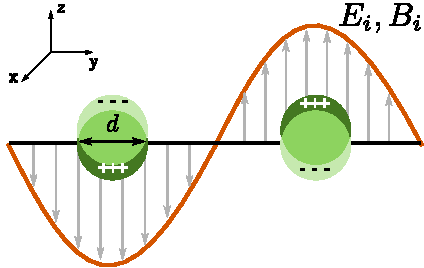
\includegraphics[width=0.35\textwidth]{lspr.pdf} 
   \caption{Illustration of the localized surface plasmon resonance (LSPR) effect of a metallic nanoparticle under an electromagnetic field. }
   \label{fig:lspr}
\end{figure}

%* What is unknown, limitations and gaps
Progress in biosensor research is still predominantly made
through experimental investigations, which can often be costly and time consuming.
Computational approaches could assist the design process and play a role  
in optimizing biosensors, giving access to details that are not available in experimental settings.
For example, empirical studies showed that the sensitivity of the sensor
is highly dependent on the distance between the nanoparticle and the analyte \cite{HaesETal2004}.
These studies were complemented with models using a discrete dipole approximation (DDA),
which includes the effect of the analyte through the effective permittivity. 
Other experimental studies complemented by modeling fully ignore the presence of the target molecules.
For example, Beuwer et al.~\cite{BeuwervanHoofZijlstra2018} and Henkel et al.~\cite{HenkelETal2018} 
used a boundary element method (BEM) in studies of the sensitivity of plasmonic sensors 
relying on (at least) two metallic nanoparticles (one on the sensor and one attached to the analyte).
Explicitly including the target molecules in the model may be needed in some cases, however.
For instance, despite experimental evidence showing that LSPR sensors are sensitive enough to detect 
conformational changes of the analytes \cite{HallETal2011}, 
these simplified models are not able to capture such details.

%* Fill the gap

Even though LSPR is an optical effect, electrostatic theory
provides a good approximation in the long-wavelength limit. This work uses
the boundary integral electrostatics solver \pygbe \cite{CooperETal2016} 
to compute the extinction cross-section of metallic nanoparticles, and to study how LSPR 
response changes in the presence of a biomolecule. 
We treat Maxwell's equations quasi-statically \cite{MayergoyzZhang2007} and
explicitly represent the target biomolecules by a surface mesh built from the crystal structures. 

\pygbe is a Python implementation of continuum electrostatic theory, used
for computing solvation energy of biomolecular systems. 
It has also been used to study protein orientation near charged nanosurfaces \cite{CooperClementiBarba2015}.
The code was recently extended to allow for complex dielectric constants 
\cite{ClementiETal2017}, aiming towards the LSPR biosensing application. 
The boundary element solver in \pygbe
is accelerated algorithmically via a treecode---an $\mathcal{O}(N\log N)$ fast-summation method---and on hardware by taking advantage of graphic processing units (GPUs). 
With these features, \pygbe is able to easily handle problems with in the order of 
half a million boundary elements, or more, 
allowing for the explicit representation of the biomolecular surface.
The software is shared under the BSD 3-clause license 
and is openly developed via its repository on Github.\footnote{\url{https://github.com/barbagroup/pygbe}}
This study also follows careful reproducibility practices, and all materials necessary
to reproduce the results are publicly available in reproducibility packages.
We use the Figshare and Zenodo services to deposit the computational meshes,
input and configuration files, and file bundles corresponding to the main figures in the paper.
See the figure captions for references to the open data artifacts.

%{\color{red}  Keeping this structure here for reference until we polish better
%the introduction.

%What is known:
%\begin{itemize}
%\item Plasmonic simulations, what applications they cover, etc. (cite Matlab guy, also Garcia de Abajo, Jung+Pedersen, etc. Maybe we can even cite COMSOL here)
%\item LSPR: how does it work, what simulations are there in the literature. Talk about work from, for example, Davis or van Duyne. See page 50 of my thesis (end chapter 2).
%\end{itemize}

%What is unkown:
%\begin{itemize}
%\item all developments are trial and error
%\item no computational tools to help in the design process
%\item example: no understanding of the sensitivity of the system
%\item models that consider the nanoparticle and the analyte are extremely simplistic
%\end{itemize}

%Fill the gap:
%\begin{itemize}
%item design of a computational tool that is highly accurate to represent the biomolecule
%\end{itemize}
%}



%=============
\section{Methods}\label{sec:methods}
\subsection{Scattering of small particles} \label{sec:scattering_small}

Electromagnetic scattering is usually modelled with Maxwell's equations.
However, when the wavelength of the incoming wave is much larger than the
scatterer, these can be reduced to a \emph{quasi-static} 
first-order approximation \cite{MayergoyzZhang2007}:
%
\begin{align} \label{eq:electrostatic_scatter_E}
\nabla \cdot \mathbf{E}_{1s} &= 0 \qquad \nabla \times \mathbf{E}_{1s} = 0, \nonumber \\
\nabla \cdot \mathbf{E}_{2s} &= 0 \qquad \nabla \times \mathbf{E}_{2s} = 0, \nonumber \\
\text{with interface conditions, } \nonumber \\
(\epsilon_1\mathbf{E}_{1s} - \epsilon_2\mathbf{E}_{2s})\cdot\mathbf{n} &= (\epsilon_2-\epsilon_1)\mathbf{E}_i\cdot \mathbf{n}.
\end{align}
%
In Equation \eqref{eq:electrostatic_scatter_E}, $\mathbf{E}_{1s}$ and $\mathbf{E}_{2s}$ 
are the electric fields of the scattered wave in the nanoparticle and host regions, respectively 
(see Figure \ref{fig:part_wave}), 
$\mathbf{E}_{i}$ is the field of the incoming wave, and $\epsilon_1$ 
and $\epsilon_2$ are the permittivities.
This approximation decouples the electric and magnetic fields, neglects the magnetic field, 
and describes the electric field as a curl-free vector field.
Hence, we can reformulate Equation \eqref{eq:electrostatic_scatter_E} with a scalar potential
($-\nabla \phi_{js} = \mathbf{E}_{js}$), as follows:
%
\begin{align} \label{eq:electrostatic_scatter}
\nabla^2 \phi_{1s} &= 0 \qquad \nabla^2 \phi_{2s} = 0 \qquad\text{on $\Omega_1$, $\Omega_2$} \nonumber \\
\epsilon_1\frac{\partial\phi_{1s}}{\partial \mathbf{n}} - \epsilon_2\frac{\partial\phi_{2s}}{\partial\mathbf{n}} &= (\epsilon_2-\epsilon_1)\frac{\partial\phi_i}{\partial\mathbf{n}} \quad \phi_{1s} = \phi_{2s} \quad \text{on $\Gamma$}.
\end{align}
%
Equation \eqref{eq:electrostatic_scatter} is an electrostatic equation 
with an imposed electric field $\mathbf{E}_i$.

\begin{figure}[h] %  figure placement: here, top, bottom, or page
   \centering
   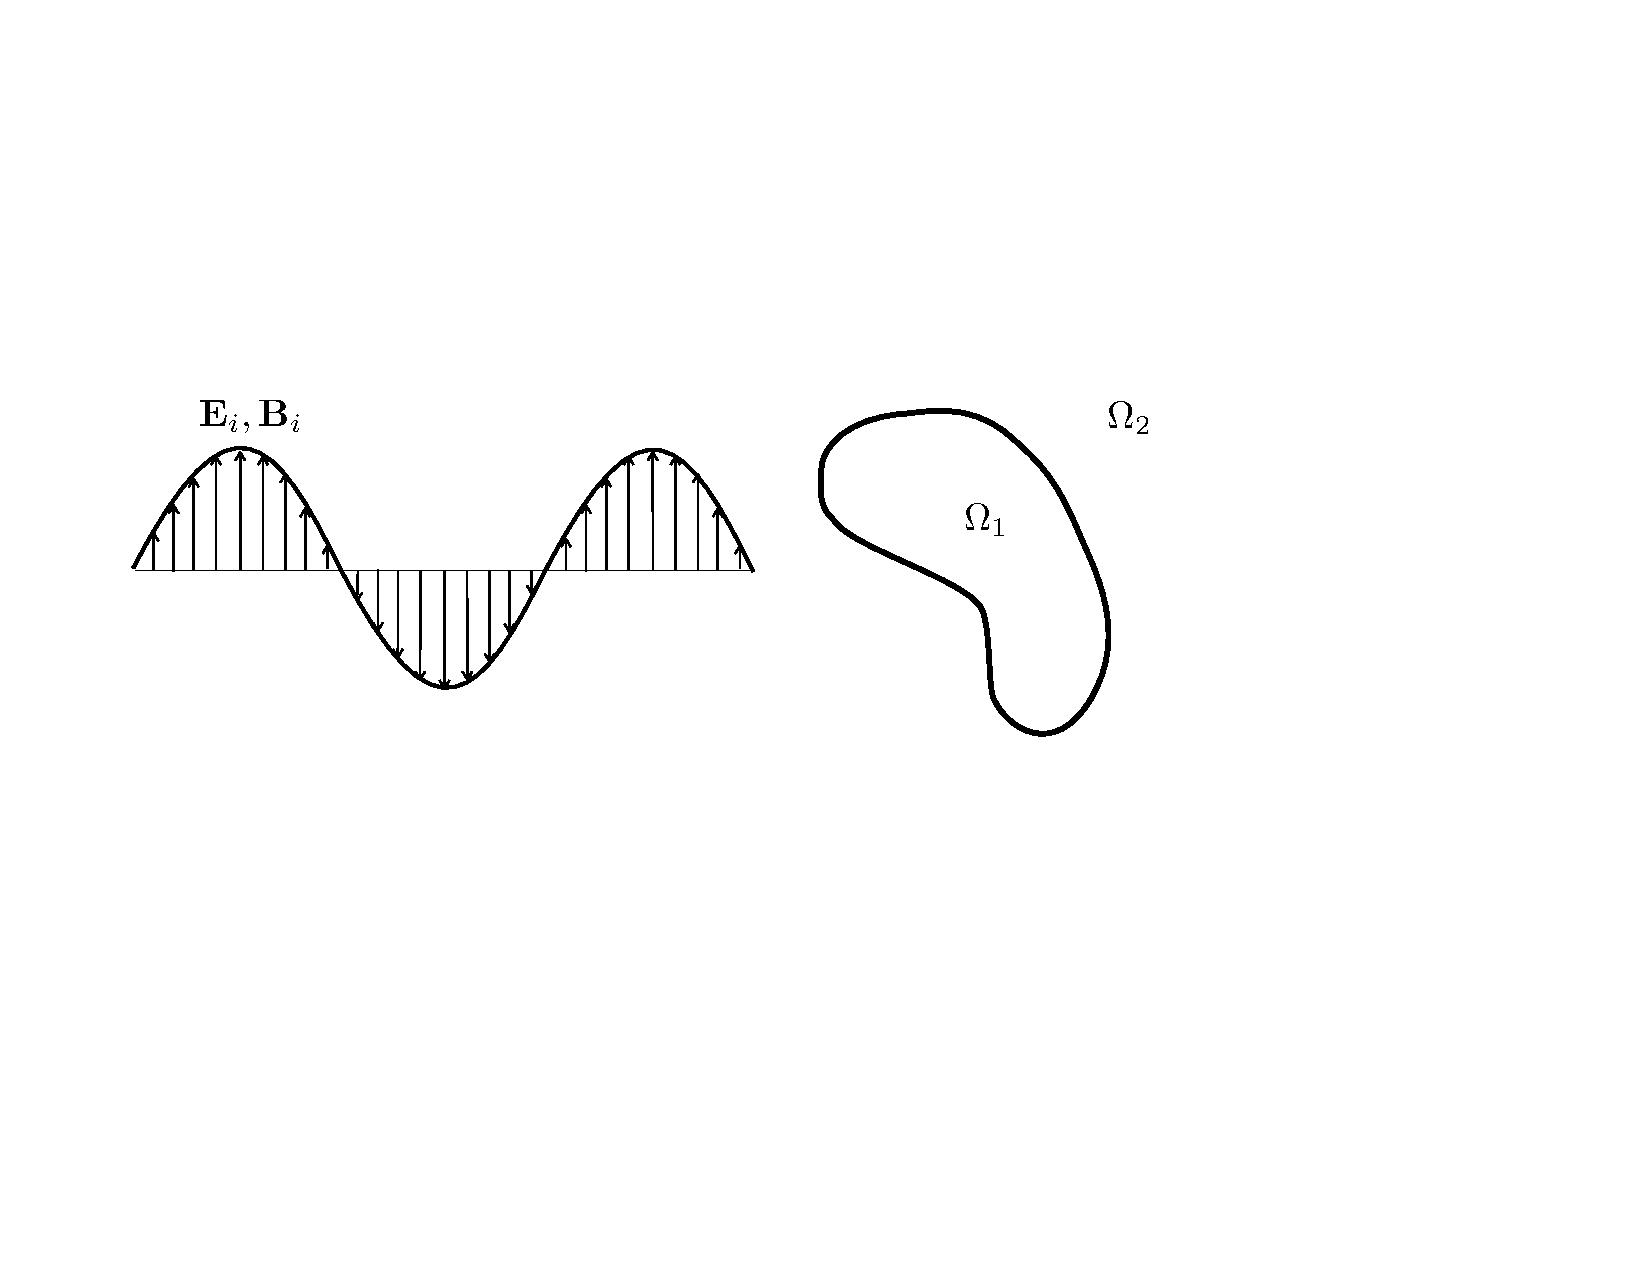
\includegraphics[width=0.45\textwidth]{particle_wave.pdf} 
   \caption{Nanoparticle under electromagnetic wave.}
   \label{fig:part_wave}
\end{figure}

\subsection{Far-field scattering} \label{sec:ff_scattering}

In LSPR, the scattered electromagnetic wave is measured by a detector located far away 
from the scatterer (nanoparticle), and plasmon resonance is identified when the energy 
detected is minimum. In the far-field limit, the scattered field
in the outside region ($\Omega_2$) is given by: 

\begin{equation} \label{eq:scat_efield_long_range}
    \mathbf{E}_{2s} = \frac{1}{4\pi\epsilon_2}k^2\frac{e^{ikr}}{r} (\mathbf{\hat{r}} \times \mathbf{p})\times\mathbf{\hat{r}}.
\end{equation} 

\noindent where $k=2\pi/\lambda$ is the wave number and $\lambda$ the wavelength, $\mathbf{\hat{r}}$ 
is a unit vector in the direction of the observation point, and $\mathbf{p}$ is
the dipole moment.
From a different approach, we can also obtain the scattered field using the forward-scattering amplitude 
\cite{Jackson}:

\begin{equation} \label{eq:scat_efield_fwa}
    \mathbf{E}_{2s}(\mathbf{r})_{r\to\infty} = \frac{e^{ikr}}{r} \mathbf{F}(\mathbf{k},\mathbf{k}_0),
\end{equation}

\noindent where $\mathbf{F}$ is the forward-scattering amplitude, $\mathbf{k}$ is the 
scattered wave vector in the direction of propagation, and $\mathbf{k}_0$ the 
wave vector of the incident field. 

\subsection{Extinction cross-section and Optical theorem} \label{sec:cext_ot}

The extinction cross-section ($C_\text{ext}$) is a measure of the energy that 
does not reach the detector, either because of scattering in other directions,
or absorption. This quantity is defined as the ratio of the lost energy and 
the intensity of the incoming wave, and has units of area. When there is 
resonance of plasmons, the extinction cross-section should peak.

On the other hand, the optical theorem relates the extinction cross-section with 
the forward-scattering amplitude. 
The traditional expression for this relationship applies for non-absorbing media 
\cite{MayergoyzZhang2007, Jackson}, however, it was corrected for absorbing media 
by Mishchenko \cite{Mishchenko2007}, giving the following expression:

\begin{equation} \label{eq:cext_fwa}
    C_\text{ext} = \frac{4\pi}{k^\prime} \operatorname{Im} \left[ \frac{\mathbf{\hat{e}}_i}{|\mathbf{E}_i|}\mathbf{F}(\mathbf{k}=\mathbf{k}_0, \mathbf{k}_0) \right].
\end{equation}


{\color{red}{Chris in Mishenko 2007 paper the equation is not exactly the same 
(look eq 87 in paper), do you have that derivation? How you got to the eq 7.22 
 in your thesis?.}\textcolor{blue}{I'll check this}}


Here, $k^\prime$ is the real part of the complex wave number. 

\begin{equation}
    k = k^\prime + ik^{\prime\prime} = \frac{2\pi}{\lambda} n,
\end{equation}

and $n$ is the refraction index of the host medium.

Combining Equations \eqref{eq:scat_efield_long_range} and \eqref{eq:scat_efield_fwa},
we can compute the forward-scattering amplitude to then obtain the extinction cross-section 
with Equation \eqref{eq:cext_fwa}


\subsection{The boundary element method} \label{sec:lspr_bem}

\subsubsection{Electrostatic potential under an electric field}

\paragraph{Integral formulation}

Using Green's second identity, the system of partial differential equations 
in Equation \eqref{eq:electrostatic_scatter_E} can be rewritten as a system 
of boundary integral equations. Evaluating on the surface $\Gamma$, the system
becomes
%
\begin{align} \label{eq:integral_eq_lspr_nobc}
\frac{\phi_{1s,\Gamma}}{2}+ K_{L}^{\Gamma}(\phi_{1s,\Gamma}) - V_{L}^{\Gamma} \left(\frac{\partial}{\partial \mathbf{n}}\phi_{1s,\Gamma} \right) = 0&  \nonumber \\
\frac{\phi_{2s,\Gamma}}{2} - K_{L}^{\Gamma}(\phi_{2s,\Gamma}) + V_{L}^{\Gamma} \left( \frac{\partial}{\partial \mathbf{n}} \phi_{2s,\Gamma} \right) = 0&,
\end{align}
%
where $V$ and $K$ are the single and double layer operators, respectively:
%
\begin{equation}\label{eq:single_layer}
V^{\mathbf{r}_\Gamma}_L (\psi(\mathbf{r}_\Gamma)) = \int_\Gamma \psi(\mathbf{r}'_\Gamma) G_L(\mathbf{r}_\Gamma, \mathbf{r}'_\Gamma) \text{d} \Gamma.
\end{equation}

\begin{equation}\label{eq:double_layer}
K^{\mathbf{r}_\Gamma}_L (\psi(\mathbf{r}_\Gamma)) = \int_\Gamma \psi(\mathbf{r}'_\Gamma) \frac{\partial}{\partial \mathbf{n}}G_L(\mathbf{r}_\Gamma, \mathbf{r}'_\Gamma) \text{d} \Gamma.
\end{equation}
%

\textcolor{red}{Chris should{t the $d\Gamma$ have a prime?}

Here, $G_L$ is the free space Green's function of the Laplace equation
%
\begin{equation}
G_L(\mathbf{r},\mathbf{r}') = \frac{1}{4\pi|\mathbf{r}-\mathbf{r}'|}
\end{equation}

Applying the interface conditions of Equation \eqref{eq:electrostatic_scatter},
leads to:
%
\begin{align} \label{eq:integral_eq_lspr}
\frac{\phi_{1s,\Gamma}}{2}+ K_{L}^{\Gamma}(\phi_{1s,\Gamma}) - V_{L}^{\Gamma} \left(\frac{\partial}{\partial \mathbf{n}}\phi_{1s,\Gamma} \right) = 0&  \nonumber \\
\frac{\phi_{1s,\Gamma}}{2} - K_{L}^{\Gamma}(\phi_{1s,\Gamma}) + \frac{1}{\epsilon_2}V_{L}^{\Gamma} \left( \epsilon_1 \frac{\partial}{\partial \mathbf{n}} \phi_{1s,\Gamma} - (\epsilon_2-\epsilon_1) \frac{\partial}{\partial \mathbf{n}} \phi_{i,\Gamma} \right) = 0& \quad \text{on $\Gamma$.}
\end{align}

%The weak formulation of Laplace equation with test function $w$:

%\begin{equation} \label{eq:lap_weak}
%\int_\Omega \nabla^2 \phi(\mathbf{r}_\Omega') w(\mathbf{r}_\Omega') \text{d} \Omega^\prime= 0.
%\end{equation}

%\noindent where the evaluation point is $\mathbf{r}_\Omega$ a location in the domain $\Omega$.

%If we use the Laplace's free-space Green's function as the test function $w$ we
%get:

%\begin{equation} \label{eq:lap_weak2}
%\int_\Omega \nabla^2 \phi(\mathbf{r}'_\Omega) G_L(\mathbf{r}_\Omega,\mathbf{r}'_\Omega) \text{d} \Omega^\prime= 0.
%\end{equation}

%Manipulating the integrand using the product rule and later the divergence 
%theorem, we get:

%\begin{equation} \label{eq:lap_bie_dom}
%\phi(\mathbf{r}_\Omega) = \int_\Gamma G_L(\mathbf{r}_\Omega,\mathbf{r}'_\Gamma)  \frac{\partial} {\partial \mathbf{n}} \phi(\mathbf{r}'_\Gamma)  \text{d} \Gamma^\prime - \int_\Gamma \phi(\mathbf{r}'_\Gamma)  \frac{\partial}{\partial \mathbf{n}} G_L(\mathbf{r}_\Omega,\mathbf{r}'_\Gamma) \text{d} \Gamma^\prime
%\end{equation}

%\noindent where \eqref{eq:lap_bie_dom}, $\mathbf{r}$ can be anywhere in the domain $\Omega$, 
%and $\mathbf{r}'$ runs only on the boundary $\Gamma$. This equation has a 
%singularity when $\mathbf{r}=\mathbf{r}'$. To handle thisproblem, we perform the
%integral on a surface $\Gamma'$ that is like $\Gamma$ but with a hemisphere of 
%radius $\varepsilon$ center at $\mathbf{r}$. We split the integrals into the part
%that we have no singularity and the part that has the hemisphere. After solving these
%equations when $\varepsilon \to 0$, equation \eqref{eq:lap_bie_dom} results in:

%\begin{equation} \label{eq:lap_bie}
%\frac{\phi(\mathbf{r}_\Gamma)}{2} +  \int_\Gamma \phi(\mathbf{r}'_\Gamma)  \frac{\partial}{\partial \mathbf{n}} G_L(\mathbf{r}_\Gamma,\mathbf{r}'_\Gamma) \text{d} \Gamma^\prime = \int_\Gamma G_L(\mathbf{r}_\Gamma,\mathbf{r}'_\Gamma)  \frac{\partial} {\partial \mathbf{n}} \phi(\mathbf{r}'_\Gamma)  \text{d} \Gamma^\prime,
%\end{equation}

%\noindent where these are Cauchy principal value integrals.

%Using the single and double layer operators:

%{\color{red} Chris, V is single layer operator but is it K the double layer one? 
%In your thesis you have that the double layer is W and you refers as K as
%"an operator" eq 2.108 and 2.112 in your thesis. Also shouldn't the $\text{d} \Gamma$
%be $\text{d} \Gamma'$? }

%\begin{equation}\label{eq:single_layer}
%V^{\mathbf{r}_\Gamma}_L (\psi(\mathbf{r}_\Gamma)) = \int_\Gamma \psi(\mathbf{r}'_\Gamma) G_L(\mathbf{r}_\Gamma, \mathbf{r}'_\Gamma) \text{d} \Gamma.
%\end{equation}

%\begin{equation}\label{eq:double_layer}
%K^{\mathbf{r}_\Gamma}_L (\psi(\mathbf{r}_\Gamma)) = \int_\Gamma \psi(\mathbf{r}'_\Gamma) \frac{\partial}{\partial \mathbf{n}}G_L(\mathbf{r}_\Gamma, \mathbf{r}'_\Gamma) \text{d} \Gamma.
%\end{equation}

%We can rewrite equation \eqref{eq:lap_bie} using the operator notation, as:

%\begin{equation} \label{eq:lap_operator}
%\left[ \frac{\mathbb{I}}{2} + K_L^{\mathbf{r}_\Gamma} \right] \left( \phi_\Gamma \right) = V_L^{\mathbf{r}_\Gamma} \left( \frac{\partial}{\partial \mathbf{n}} \phi_\Gamma \right),
%\end{equation}

%\noindent where $\mathbb{I}$ is the identity operator.

%Following the same stepps, we can rewrite the Laplace equations in eqaution
%\eqref{eq:electrostatic_scatter} as:

%
%\begin{align} \label{eq:integral_eq_lspr_nobc}
%\frac{\phi_{1s,\Gamma}}{2}+ K_{L}^{\Gamma}(\phi_{1s,\Gamma}) - V_{L}^{\Gamma} \left(\frac{\partial}{\partial \mathbf{n}}\phi_{1s,\Gamma} \right) = 0&  \nonumber \\
%\frac{\phi_{2s,\Gamma}}{2} - K_{L}^{\Gamma}(\phi_{2s,\Gamma}) + V_{L}^{\Gamma} \left( \frac{\partial}{\partial \mathbf{n}} \phi_{2s,\Gamma} \right) = 0& \quad \text{on $\Gamma$,}
%\end{align}

%Applying the interface conditions of Equation \eqref{eq:electrostatic_scatter},
%we get:

%\begin{align} \label{eq:integral_eq_lspr}
%\frac{\phi_{1s,\Gamma}}{2}+ K_{L}^{\Gamma}(\phi_{1s,\Gamma}) - V_{L}^{\Gamma} \left(\frac{\partial}{\partial \mathbf{n}}\phi_{1s,\Gamma} \right) = 0&  \nonumber \\
%\frac{\phi_{1s,\Gamma}}{2} - K_{L}^{\Gamma}(\phi_{1s,\Gamma}) + \frac{1}{\epsilon_2}V_{L}^{\Gamma} \left( \epsilon_1 \frac{\partial}{\partial \mathbf{n}} \phi_{1s,\Gamma} - (\epsilon_2-\epsilon_1) \frac{\partial}{\partial \mathbf{n}} \phi_{i,\Gamma} \right) = 0& \quad \text{on $\Gamma$.}
%\end{align}


\paragraph{Discretization and linear system}


We discretize the surface into flat triangles, and assume that  $\phi$ and 
$\partial \phi/\partial \mathbf{n}$ are constant within each panel. Then, we can
write the layer operators in their discretized form:
%
\begin{align} \label{eq:layers_disc}
V_{L,\text{disc}}^{\mathbf{r}_\Gamma} \left( \frac{\partial}{\partial \mathbf{n}} \phi(\mathbf{r}_{\Gamma}) \right) &= \sum_{j=1}^{N_p} \frac{\partial}{\partial \mathbf{n}} \phi(\mathbf{r}_{\Gamma_j}) \int_{\Gamma_j} G_L(\mathbf{r}_\Gamma,\mathbf{r}_{\Gamma_j})  \mathrm{d} \Gamma_j  \nonumber \\
K_{L,\text{disc}}^{\mathbf{r}_\Gamma}(\phi(\mathbf{r}_{\Gamma})) &=  \sum_{j=1}^{N_p}\phi(\mathbf{r}_{\Gamma_j})\int_{\Gamma_j} \frac{\partial}{\partial \mathbf{n}} \left[ G_L(\mathbf{r}_\Gamma,\mathbf{r}_{\Gamma_j}) \right]\mathrm{d} \Gamma_j
\end{align}
%
\noindent where $N_p$ is the number of discretization elements of $\Gamma$, 
and $\phi(\mathbf{r}_{\Gamma_j})$ and $\frac{\partial}{\partial \mathbf{n}} 
\phi(\mathbf{r}_{\Gamma_j})$ are the values of $\phi$ and 
$\frac{\partial \phi}{\partial \mathbf{n}}$ on panel $\Gamma_j$.
Then, using centroid collocation, we can write equation \eqref{eq:integral_eq_lspr} in matrix form as:
%
 \begin{equation} \label{eq:matrix_lspr}
 \left[
    \begin{matrix} 
       \frac{1}{2} + K_{L}^{\Gamma} & -V_{L}^{\Gamma}  \vspace{0.2cm} \\
       \frac{1}{2} - K_{L}^{\Gamma} &  \frac{\epsilon_1}{\epsilon_2} V_{L}^{\Gamma}  \vspace{0.2cm} 
    \end{matrix}
    \right] \left[ 
    \begin{matrix} 
       \phi_{1s,\Gamma} \vspace{0.2cm} \\
       \frac{\partial}{\partial \mathbf{n}} \phi_{1s,\Gamma} \vspace{0.2cm}
    \end{matrix} 
     \right] =   
    \left[
    \begin{matrix} 
       0 \\
       V_{L}^{\Gamma} \left(\frac{\epsilon_2-\epsilon_1}{\epsilon_2}\right) \frac{\partial\phi_i}{\partial\mathbf{n}} \vspace{0.2cm} 
    \end{matrix}
    \right]
 \end{equation}
%
\noindent where the elements of the matrix are
%
\begin{align} \label{eq:layers_element}
V_{L,ij}^{\Gamma} &= \int_{\Gamma_j} G_L(\mathbf{r}_{\Gamma_i},\mathbf{r}_{\Gamma_j})  \mathrm{d} \Gamma_j \nonumber \\
K_{L,ij}^{\Gamma} &= \int_{\Gamma_j} \frac{\partial}{\partial \mathbf{n}} \left[ G_L(\mathbf{r}_{\Gamma_i},\mathbf{r}_{\Gamma_j}) \right]\mathrm{d} \Gamma_j
\end{align}
%
\noindent with $\mathbf{r}_{\Gamma_i}$ being at the center of panel $\Gamma_i$.

\paragraph{Integral evaluation}

We evaluate the integrals in Equation \eqref{eq:layers_element} with Gauss quadrature
rules. However, the $1/r$ singularity of the Green's function is a
problem to obtain good accuracy when the integral is 
singular or near-singular. Therefore, we define three different regions:

\emph{Singular integrals:} If the collocation point is in the integrated panel,
there is a singularity that is difficult to resolve with standard
Gauss integration schemes. In this case, we use a semi-analytical technique 
\cite{HessSmith1967,ZhuHuangSongWhite2001} that places $N_k$ quadrature nodes on the 
edges of the triangle.

\emph{Near-singular integrals:} If the collocation point is close to the integration panel,
the integrand has a high gradient, and high-order quadrature rules are required. 
We use the representative length of the integrated triangle ($L = \sqrt{2\cdot\text{Area}}$)
to define a threshold of the \emph{close-by} region, for example, when the integration panel 
is $2L$ or less away from the collocation point. For near-singular integrals, we use 
$K_{fine}=19, 25 \; or \; 37$ points per triangle. 

\emph{Far-away integrals:} When the distance between the collocation point and the integration
panel is beyond the threshold, they are considered to be far-away. 
At this point, the integrand is smooth enough that we obtain good 
accuracy with low order integration, for example, with 
$K=1, 3 \; or \; 4$ Gauss quadrature points per boundary element. 

\subsubsection{Boundary integral expression of the dipole moment}

As shown in Equation \eqref{eq:scat_efield_long_range}, the scattered electric 
field in the far-away limit depends on the dipole moment. The dipole moment is 
defined as 

%
\begin{equation} \label{eq:dipole_def}
\mathbf{p} = \int_\Omega \mathbf{r} \rho \text{d}\Omega,
\end{equation}

Rewriting this equation using Gauss's law we obtain
%
\begin{equation} \label{eq:dipole_def_gauss}
\mathbf{p} = -\epsilon_2\int_\Omega \mathbf{r} \nabla^2 \phi_{2s} \text{d}\Omega.
\end{equation}


{\color{red} Here is where we need to sort out the sign problem in equations and 
how we write the derivation. Will fix when we talk with Chris}
\textcolor{blue}{need to check this, and include the whole derivation}

\subsection{Acceleration startegies} \label{sec:acc_strategies}

The main downside of the Boundary Element Method (\bem) is that it generates dense matrices
after discretization. Solving the linear system using
Gaussian elimination requires $\O{N^3}$ computations and $\O{N^2}$ storage, whereas for a
Krylov-subspace iterative solver, like the Generalized Minimal Residual Method (\gmres),
computations drop to $\O{N^2}$ because they are dominated by a matrix-vector 
product. This makes \bem a good approach for problems with no more than a few thousand boundary elements,
which is far from the mesh sizes required for real applications. 

Since we are using Gaussian quadrature and collocation, the matrix-vector product
becomes an N-body problem, where the Gauss nodes act as centers of mass (\emph{sources}), and we evaluate
the potential at the collocation points (\emph{targets}).
To overcome the $\O{N^2}$ scaling,
we accelerate the matrix-vector product using a Treecode algorithm \cite{BarnesHut1986,DuanKrasny2001}, 
which is a fast-summation algorithm capable of reducing $\O{N^2}$
computational patterns 
%
\begin{equation} \label{eq:summation}
V(\mathbf{x}_i) = \sum_{j=1}^{N} q_j \psi(\mathbf{x}_i, \mathbf{y}_j) 
\end{equation}
%
\noindent to a computational complexity of $\O{N \log N}$. In Equation \eqref{eq:summation} 
$q_j$ is the weight, $\psi$ the kernel, $\mathbf{y}_j$ the locations of sources and 
$\mathbf{x}_i$ the locations of targets.

The Treecode groups sources geometrically in boxes of an octtree, which is built making
sure that no box in the lowest level has more than $N_\text{crit}$ sources. Then, if a group of
sources is far away from a target, their influence is aggregated in an expansion center,
and the target interacts with the box, rather than with each source independently.
On the other hand, if the group of targets is too close, the Treecode queries the child
boxes. If the box has no children and still is not far enough, the interaction is 
performed directly. The threshold to decide if a box is far enough is called the multipole-
acceptance criterion (MAC):
%
\begin{equation}
\theta > \frac{r_b}{r},
\end{equation}
%
where $r_b$ is the box size and $r$ the distance between the box center and the target.
Common values of $\theta$ are $1/2$ and $2/3$.
To approximate the contribution of the sources, we use Taylor expansions
of order $P$.
The Treecode allows us to control accuracy of the approximation by modifying $\theta$ and $P$.
Further details of the Treecode implementation in \pygbe can be found in \cite{CooperBarba-share154331,CooperBardhanBarba2013}.
 

%=============
\section{Results} \label{sec:results}
%!TEX root = ClementiCooperBarba2018.tex

\subsection{Grid convergence and verification with an isolated silver nanoparticle} \label{sec:verification}

\noindent In the long-wavelength limit, the electrostatic approximation applies and
the electromagnetic scattering of a small spherical particle can be modeled
by a sphere in a constant electric field. 
Figure \ref{fig:np_elec_field} illustrates this scenario.

%
\begin{figure}[h] %  figure placement: here, top, bottom, or page
   \centering
   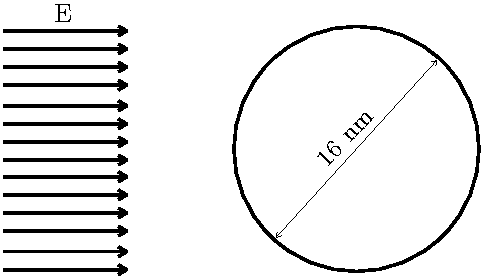
\includegraphics[width=0.3\textwidth]{sphere_field_8nm.pdf} 
   \caption{Spherical nanoparticle in a constant electric field.}
   \label{fig:np_elec_field}
\end{figure}
%

This model problem has an analytical solution, which allows us to compare with
the numerical calculations of the extinction cross-section obtained with \pygbe,
for code verification and grid-convergence analysis.
Mishchenko \cite{Mishchenko2007} derived the following analytical result, 
valid for lossy mediums:
%
\begin{equation} 
    C_\text{ext} = \frac{4\pi a^3}{k^\prime} \operatorname{Im}\left(k^2 
                    \frac{\epsilon_p/\epsilon_m -1}{\epsilon_p/\epsilon_m +2}\right),
    \label{eq:an_sol}
\end{equation}
%
Here, $a$ is the radius of the sphere, $k$ is the complex wave number ($k=k^\prime +i k^{\prime\prime}$), $\epsilon_p$ 
is the dielectric constant of the particle, and $\epsilon_m$ is the dielectric constant
of the host medium. If the medium is not lossy, then $k^{\prime\prime}=0$ and $k=k^\prime$.

We completed a grid-convergence study of \pygbe for the extinction
cross-section of a spherical silver nanoparticle of radius 8 nm immersed in water,
under a z-polarized electric field with a wavelength of 380 nm and intensity of 
$-0.0037 e/({\AA}^2 \, \epsilon_0)$. In these conditions, water has a dielectric
constant of $1.7972 \, + \, 8.5048^{-09}i$ \cite{JohnsonChristy1972} and silver of
$-3.3877 \, + \, 0.1922i$ \cite{HaleQuerry1972}. 
Table \ref{table:quadparams1} lists the Gauss quadrature points for each type of element. 
The threshold parameter defining the near-singular region was 0.5 (refer to the \pygbe documentation, under ``Parameter file format'').

\begin{table}[h]
    \centering
    \caption{\label{table:quadparams1} Isolated silver nanoparticle: Gauss quadrature points; 
    $K$ and $K_{fine}$ are per element; $Nk $ is per element edge (semi-analytical integration). } 
    \begin{tabular}{l l}
    \hline%\toprule
     distant elements: & $K=4$ \\
     near-singular integrals:   & $ K_{fine}=37$ \\
     singular elements:  & $Nk =9$ \\
    \hline%\bottomrule
    \end{tabular}
\end{table}


\begin{table}[h]
    \centering
    \caption{\label{table:treeparams1} Isolated silver nanoparticle: treecode and solver parameters.} 
    \begin{tabular}{l l}
    \hline%\toprule
    treecode order of expansion: & $P=15$\\
    MAC                                         & $\theta=0.5$\\
    GMRES tolerance                    & $10^{-5}$\\
    \hline%\bottomrule
    \end{tabular}
\end{table}

The results are shown in Figure \ref{fig:error_sphere_Ag}, where the mesh sizes are
512, 2048, 8192, and 32768 elements. 
The analytical solution with equation \eqref{eq:an_sol} is $C_{ext} = 1854.4765$ nm$^2$, 
and the errors are as shown in Table \ref{table:err_iso_sphere}.
The observed order of convergence is $0.98$, and the $1/N$ slope in Figure \ref{fig:error_sphere_Ag}
is an indication that the meshes are correctly resolving the numerical solutions with \pygbe. 


\begin{figure}[h] %  figure placement: here, top, bottom, or page
   \centering
   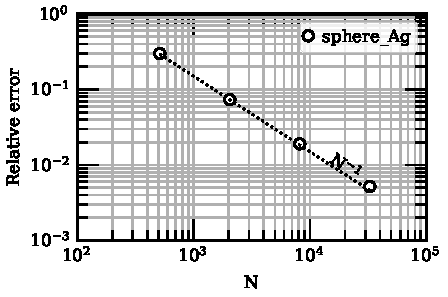
\includegraphics[width=0.45\textwidth]{convergence_sph_Ag_R8_w=380.pdf} 
   \caption{Grid-convergence study of extinction cross-section of a spherical silver
            nanoparticle.}
   \label{fig:error_sphere_Ag}
\end{figure}



\begin{table}[h]
    \centering
    \caption{\label{table:err_iso_sphere} Percentage error of isolated silver sphere.} 
    \begin{tabular}{c c}
    \hline%\toprule
    N & \% error \\
    \hline%\midrule
     $512$ & $29.86$ \\
     $2048$ & $7.33$ \\
     $8192$ & $1.9$ \\
     $32768$ & $0.52$ \\
    \hline%\bottomrule
    \end{tabular}
\end{table}

We further verified our implementation computing the extinction cross-section of the 
isolated sphere for a range of wavelengths, presented in Figure \ref{fig:verif_sphere}. 
The mesh in these simulations had $N=32768$, which yields errors below $2\%$ in Table \ref{table:err_iso_sphere}.
The values of dielectric constants for each wavelength were obtained by interpolation of 
experimental data \cite{JohnsonChristy1972, HaleQuerry1972}.

\begin{figure}[h] %  figure placement: here, top, bottom, or page
   \centering
   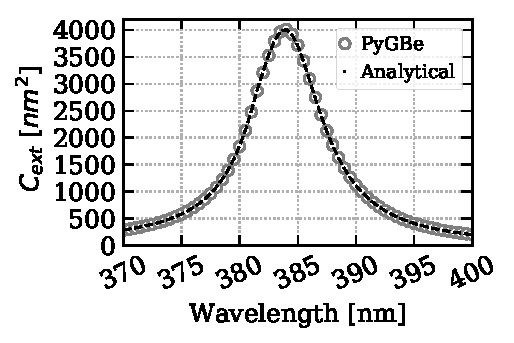
\includegraphics[width=0.45\textwidth]{silver_NP_verification.pdf} 
   \caption{Extinction cross-section as a function of wavelength for a $8 \, nm$
            silver sphere immersed in water.}
   \label{fig:verif_sphere}
\end{figure}

Figure \ref{fig:verif_sphere} shows good agreement between simulations and analytical results, proving
that \pygbe is accurately representing the mathematical model. The 
peak in the extinction cross-section indicates that the plasmons of the metallic
nanoparticle are resonating with the incoming electric field.


\subsection{LSPR response to BSA} \label{sec:lspr_response}

Localized Surface Plasmon Resonance (LSPR) biosensors detect a target molecule by monitoring
plasmon resonance frequency shifts of metallic nanoparticles, in presence of an analyte \cite{WilletsVandyune2007}.
In this section, we use our BEM approach to model the response of LSPR biosensors.
We consider a spherical silver nanoparticle, and compute the extinction cross-section placing 
bovine serum albumina (BSA) proteins (PDB code: 4FS5) in different locations.
The BSA mesh was generated using the open source software Nanoshaper \cite{Nanoshaper}. 
Nanoshaper takes as inputs the atomic coordinates and radii, which were 
extracted from a \texttt{pqr} file generated with \texttt{pdb2pqr} \cite{Dolinsky04},
 using the built-in \texttt{amber} force field.

\subsubsection{Grid-convergence study} \label{sec:bsa_convergence}
To guarantee an accurate numerical solution, we performed a grid-convergence 
analysis of the system sketched in Figure \ref{fig:setup_conv}. 
Since we compute the extinction cross-section of the spherical nanoparticle only, we 
set a fixed mesh density for the protein and refined the mesh of the
sphere (meshes of 512, 2048, 8192 and 32768 elements). We found that the protein meshed with two
triangles per ${\AA}^2$ was fine enough for the convergence analysis, resulting in $N_{prot} = 98116$ elements. 


\begin{figure}[h] %  figure placement: here, top, bottom, or page
   \centering
   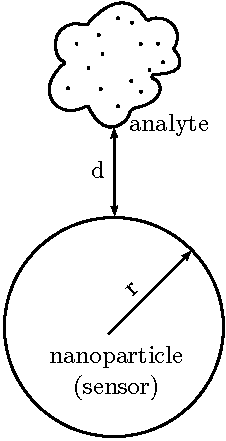
\includegraphics[width=0.15\textwidth]{protein_sphere_sketch.pdf} 
   \caption{Setup for convergence analysis of the response calculation.}
   \label{fig:setup_conv}
\end{figure}

These tests used the conditions and parameters for the isolated sphere simulation
presented in Section \ref{sec:verification}. The protein dielectric constant was
$2.7514 + 0.2860i$, which we extracted from the 
functional relationship provided by Phan, et al. \cite{PhanETal2013}, and the 
distance between the sensor and the analyte was $d=1 \, nm$. BSA was oriented such that
its dipole moment was aligned with the y-axis. The error calculations for Figure \ref{fig:error_sphere-bsa}
and Table \ref{table:err_bsa_sensor} use the Richardson extrapolated value of extinction cross-section as a
reference, $C_{ext}= 1778.7259 \, nm^2$.


\begin{figure}[h] %  figure placement: here, top, bottom, or page
   \centering
   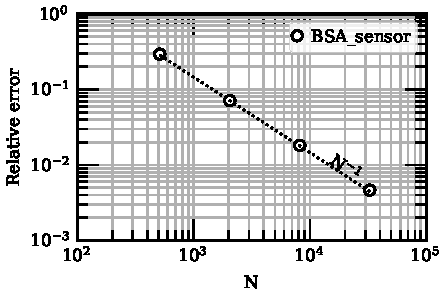
\includegraphics[width=0.45\textwidth]{convergence_bsa_sensor_R8_d=1_w=380.pdf} 
   \caption{Grid-convergence study of extinction cross-section of a spherical silver
            nanoparticle with a BSA protein at $d=1 \, nm$.}
   \label{fig:error_sphere-bsa}
\end{figure}

The observed order of convergence is $0.99$, and 
Figure \ref{fig:error_sphere-bsa} shows that the error decays with the number
of boundary elements ($1/N$), which is consistent with our verification 
results in Section \ref{sec:verification}. This proves that the
numerical solutions computed with \pygbe are correctly resolved by the meshes.
Also, the percentage errors for the different meshes are presented in Table. \ref{table:err_bsa_sensor}.

\begin{table}[h]
    \centering
    \caption{\label{table:err_bsa_sensor} Percentage error of BSA-sensor sytem (Fig.\ref{fig:setup_conv}) .} 
    \begin{tabular}{c c}
    \hline%\toprule
    N & \% error \\
    \hline%\midrule
     $512$ & $29.39$ \\
     $2048$ & $7.13$ \\
     $8192$ & $1.82$ \\
     $32768$ & $0.46$ \\
    \hline%\bottomrule
    \end{tabular}
\end{table}

\subsubsection{Resonance frequency shift calculations} \label{sec:bsa_shift}

We studied the LSPR response as a function of the wavelength in the presence 
of the BSA. To optimize run-times without compromising accuracy, we used a relaxed
set of parameters, where the protein mesh density was one element per
${\AA}^2$ ($N_{prot}=45140$) and the sphere mesh had $N_{sensor}=32768$. Integrals used
$K=4$ Gauss quadrature points for far-away elements, 
$K_{fine} = 19$ Gauss quadrature points in elements with near singular integrals,
and $Nk = 9$ Gauss quadrature points per triangle edge for the semi-analytical integration in the 
singular elements. The treecode used a Taylor expansion of order $P=6$ and a multipole-acceptance
criterion of $\theta=0.5$ . The GMRES tolerance was set to $10^{-3}$. 
This parameter choice resulted in a percentage error of $\sim\%0.6$
and the time of each computation was approximately $7.5 \, \text{min}$ in a \texttt{NVIDIA Tesla K40 GPU}
card when we have only one protein (when two proteins are present the time per run
is $\sim 15 \, \text{min}$). 

Figure \ref{fig:display_z} sketches the setup of the simulations, with two proteins placed 
$d=1 \, nm$ away from a spherical silver nanoparticle, along the z-axis.
The position of the BSA in the $+z$ axis was the same as the convergence analysis in 
Section \ref{sec:bsa_convergence}, whereas the BSA in the $-z$ position comes from a 180$^\circ$ 
solid rotation of the BSA in $+z$ about the y-axis.
We performed calculations for wavelengths between $382 \, nm$ and $387 \, nm$, every $0.25 \, nm$,
which are around the peak seen in Figure \ref{fig:verif_sphere}.

Figure \ref{fig:2pz_response} shows the variation of the extinction cross-section
with respect to wavelength for the isolated nanoparticle ($d=\infty$) and with
BSA proteins placed $d=1 \, nm$ away. 
Results present a red-shift ($0.5 \, nm$) in the resonance frequency due to the
presence of the BSA analytes.


\begin{figure}[h] %  figure placement: here, top, bottom, or page
   \centering
    %since we have dots in the names we need to enclose what is before the 
    %extension in { }
   \includegraphics[width=0.45\textwidth]{{2pz_00_ef-0.0037_R8nm}.pdf} 
   \caption{Extinction cross-section as a function of wavelength for a $8 \, nm$
            silver sphere immersed in water with two BSA proteins placed at
            $\pm 1 \; nm$ away from the surface in the z-direction, and at
            infinity (no protein).}
   \label{fig:2pz_response}
\end{figure}


To study the effect of location of the analytes, we reran simulations placing the 
BSA proteins along the x- and y-axis, at $\pm 1 \; nm$, as sketched by Figure \ref{fig:display_xy}.
Figure \ref{fig:2pxy_response} shows the results obtained for x-axis and
y-axis display, respectively. 

\begin{figure}[!h] %  figure placement: here, top, bottom, or page
   \centering
   \subfloat{\includegraphics[width=0.45\textwidth]{{2px_00_ef-0.0037_R8nm}.pdf}}
   \quad 
   \subfloat{\includegraphics[width=0.45\textwidth]{{2py_00_ef-0.0037_R8nm}.pdf}} 
   \caption{Extinction cross-section as a function of wavelength for a $8 \, nm$
            silver sphere immersed in water with two BSA proteins placed at
            $\pm 1 \; nm$ away from the surface in the x-direction (top) and
             y-direction (bottom), and at infinity (no protein).}
   \label{fig:2pxy_response}
\end{figure}

\subsubsection{Sensitivity calculations} \label{sec:bsa_sensitivity}

The sensitivity of an LSPR biosensor corresponds to the relation between the size 
of the resonance frequency shift and the number of analytes bound to the sensor (through a ligand).
Experiments show that the distance between the nanoparticle and the analyte largely
affects the sensitivity of the sensor, to the point that
targets placed $15nm$ away from the surface are very hard to detect \cite{HaesETal2004}.
This is a critical issue, considering that common ligands (for example, antibodies) are
larger than $15nm$. Figure \ref{fig:dist_response} 
shows how the peak varies with the distance at which the analytes ($+z$ and $-z$) are placed.  
In particular, we see a shift of $0.25 \, nm$ when $d=2 nm$ to $0.75 nm$ when the 
analytes are placed at $d=0.5 \, nm$. The parameters used in this case remain 
the same as the ones used in Figures \ref{fig:2pz_response} and \ref{fig:2pxy_response} .


\begin{figure}[h] %  figure placement: here, top, bottom, or page
   \centering
   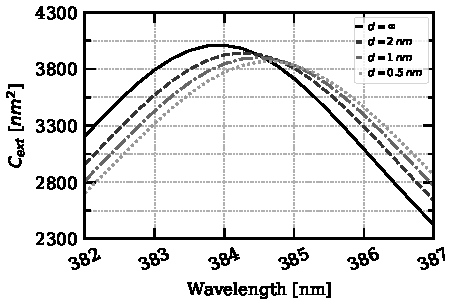
\includegraphics[width=0.45\textwidth]{2pz_lspr_response.pdf} 
   \caption{Extinction cross-section as a function of wavelength for a $8 \, nm$
            silver sphere immersed in water with two BSA proteins placed at
            $2, \, 1 \, \text{and} \, 0.5 \, nm$ away from the surface in the 
            z-direction, and at infinity (no protein)}
   \label{fig:dist_response}
\end{figure}

\begin{figure*}[] %  figure placement: here, top, bottom, or page
   \centering
   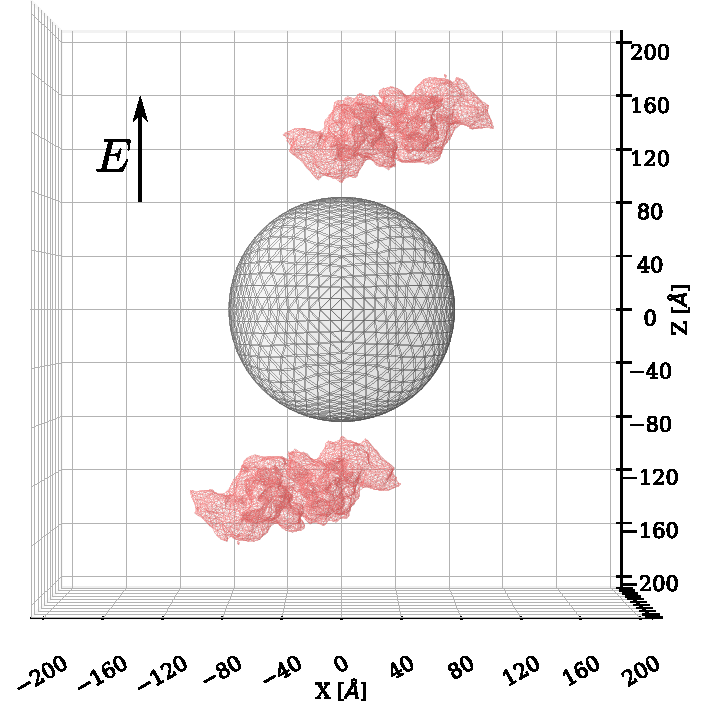
\includegraphics[width=0.65\textwidth]{2prot_1nm_z_R8nm.pdf} 
   \caption{Sensor protein display: BSA located at $\pm 1 \, nm$ of the 
            nanoparticle in the z-direction}
   \label{fig:display_z}
\end{figure*}

\begin{figure*}[]

   \centering
   \subfloat{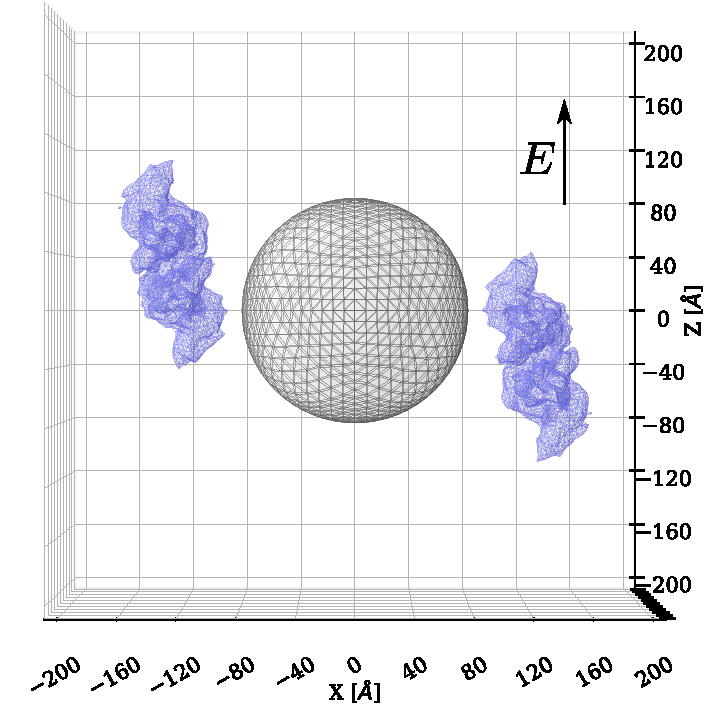
\includegraphics[width=0.65\textwidth]{2prot_1nm_x_R8nm.pdf}} 
%   \caption{Sensor protein display: BSA located at 1 nm of the nanoparticle in the
%            x-direction}
   %\label{fig:display_x}
    \vfill
   \subfloat{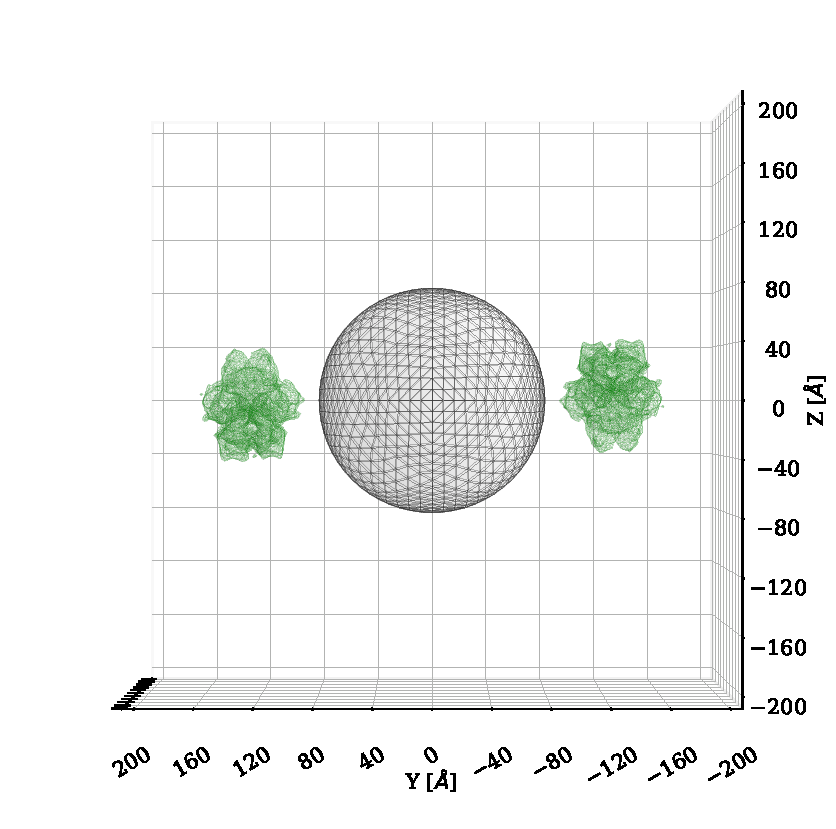
\includegraphics[width=0.65\textwidth]{2prot_1nm_y_R8nm.pdf}} 
%   \caption{Sensor protein display: BSA located at 1 nm of the nanoparticle in the
%            y-direction}
    \caption{Sensor protein display: BSA located at $\pm 1 \, nm$ of the nanoparticle in the
            x-direction (top) and y-direction (bottom)}
    \label{fig:display_xy}
\end{figure*}

\subsection{Reproducibility} \label{sec:repro}

We believe in reproducibility practices. To facilitate the replication of our results, 
we consistently release our code and data with every publication. \pygbe is developed and 
shared \footnote{\url{https://github.com/barbagroup/pygbe}} under the BSD3-clause 
license and the development repository is available on Github. We also release
all of the data and scripts needed to run the numerical simulations in this work, 
as well as the post-processing scripts to reproduce the figures in this paper. To be consistent with our open-source policy, we release a \textit{reproducibility package} for each of the results prensented in
this paper. {\color{red} explain location and which figure correspond to each package
after finished repropack}



%=============
\section{Discussion} \label{sec:discussion}
\subsection{LSPR response to BSA}

Figure \ref{fig:2pz_response} shows a red shift of the plasmon resonance frequency peak in presence of the BSA protein.
This result agrees with experimental observations
\cite{TangETal2010, RaphaelETal2013}. Moreover, we observe a decrement of 
the peak which is also present in the results of Tang, et al. \cite{TangETal2010}.
Both results, the red-shift and the decrement of the peak in the presence of 
the proteins, indicate that our boundary element method approach using electrostatic
approximation, is capable of reproducing the characteristic resonance frequency 
shift in LSPR biosensors.

The effect of placing the proteins in a direction that is not aligned with the incoming electric field
is presented by Figure \ref{fig:2pxy_response}. In both cases we can observe that the shift is negligible, 
as the shift is smaller than the resolution between wavelengths ($< 0.25 nm$), resulting in an
effectively zero-shift. These findings are consistent with 
the fact that we have a z-polarized electric field. Having a z-polarized electric
field implies that the cloud of electrons will be smaller in the x and y direction.
\textcolor{blue}{(we need to redo this explanation)}
Therefore, the effect of the analyte in those locations results insignificant. 

In Figure \ref{fig:dist_response} we can observe how the distance between the sensor 
and the analyte affects the shift in resonance frequency. As expected, the shift decays 
as the BSA moves away from the sensor, to the point that is the BSA proteins are placed
$d=2 nm$ away, the the shift is only $0.25 \, nm$. This result shows the potential of \pygbe 
and the electrostatic approach to study sensitivity versus distance.
One has to consider that detection of such
small number of analytes is not possible in experiments, however, these simulations can shine light on
potential improvements that would enhance sensitivity of LSPR biosensors, for example, by using
smaller ligands. 





\section{Conclusion}
%\input{conclusion}

In this work, we combined the implicit-solvent model of electrostatics interactions in \pygbe 
with a long-wavelength representation of LSPR response in nanoparticles. 
We extended \pygbe to work with complex-valued quantities, and added functionality to 
include an imposed electric field and compute relevant quantities 
(dipole moment, extinction cross-section). 
Previous work with \pygbe showed its suitability for computing 
biomolecular electrostatics considering solvent-filled cavities and Stern layers \cite{CooperBardhanBarba2013}, 
and for protein-surface electrostatic interactions \cite{CooperBarba2016}.
This latest extension can offer a valuable computational approach to study nanoplasnomics and aid in the design of LSPR biosensors. 
Thanks to algorithmic acceleration with a treecode, and hardware acceleration with GPUs, \pygbe is able to compute problems with half a million elements, or more, which is required to represent the molecular surface accurately.



\begin{acknowledgments}

CDC acknowledges the financial support from CONICYT through projects FONDECYT Iniciaci\'on 11160768 and Basal FB0821.
\end{acknowledgments}

% Create the reference section using BibTeX:
%\bibliographystyle{} % revtex ournal sub-style automatically sets this
\bibliography{compbio,bem,scicomp,fastmethods,biosensors} %don't leave spaces between elements, it throws error

\end{document}
